\section{Estratégias de escalabilidade}
\label{sec:escalabilidade}

\subsection{O que limita a escala hoje}

A escalabilidade de uma plataforma depende de a receita adicional de cada novo usuário superar o custo adicional de atendê-lo. A Tabela~\ref{tab:unitaria} decompõe, a partir das premissas da Atividade IX, a economia de um usuário ativo mensal no cenário-base, sem convênios.

\begin{table}[htb]
\centering
\caption{Economia por usuário ativo mensal no cenário-base (R\$/mês)}
\label{tab:unitaria}
\fontsizetable
\begin{tabularx}{\textwidth}{Y L{3.0cm}}
\toprule
\textbf{Linha} & \textbf{Valor por usuário}\\
\midrule
Receita: comissão de intermediação (10\% dos atendimentos, 10\% dos usuários) & 0,77\\
Receita: assinatura PetCuida+ (5\% dos usuários) & 0,65\\
Receita: Plano Parceiro (1 clínica por 150 usuários) & 0,53\\
\textbf{Receita total} & \textbf{1,95}\\
(--) Taxas de pagamento e da loja de aplicativos & (0,32)\\
(--) Impostos (6\%) & (0,12)\\
(--) Infraestrutura e suporte & (0,30)\\
(--) Fundo de liquidação de créditos & (0,66)\\
\textbf{Contribuição por usuário ativo} & \textbf{0,55}\\
\bottomrule
\end{tabularx}
\fontetexto{cálculo dos autores a partir da Atividade IX (Apêndice A)}
\end{table}

O resultado é revelador: cada usuário adicional contribui com apenas R\$~0,55 por mês, e o fundo de liquidação de créditos (R\$~0,66 por usuário) é maior do que a contribuição líquida. Em consequência, para cobrir os custos fixos do cenário com equipe remunerada, seriam necessários cerca de 10.155 usuários ativos mensais, mesmo contando com o convênio (Atividade IX). Crescer apenas em número de usuários, sem alterar a composição da receita e do fundo, é caminho longo e frágil. As ações a seguir buscam elevar a contribuição por usuário e reduzir o custo fixo por usuário, que é a definição prática de escalar.

\subsection{Automação de processos}

\begin{table}[htb]
\centering
\caption{Processos candidatos à automação}
\label{tab:automacao}
\fontsizetable
\begin{tabularx}{\textwidth}{L{3.2cm} Y Y}
\toprule
\textbf{Processo} & \textbf{Automação proposta} & \textbf{Efeito esperado}\\
\midrule
Cadastro de clínicas e profissionais & Autocadastro de organizações e importação em lote de profissionais, funcionalidade já presente na aplicação web (até 500 linhas por arquivo) \cite{cassino2026repo}. & Onboarding de nova clínica sem trabalho manual da equipe.\\
Lembretes de vacinas e consultas & Notificações automáticas pelo calendário do animal; o custo das notificações do Firebase é nulo, segundo a Atividade IX. & Engajamento e retenção sem custo variável relevante.\\
Triagem orientativa & Fluxo por perguntas com regras fixas e encaminhamento, sem diagnóstico, com revisão veterinária da base de regras. & Menos atendimentos humanos de primeira linha.\\
Pagamentos e repasses & Conciliação automática dos pagamentos por Pix e cartão e relatório mensal de repasses às clínicas. & Menos horas de operação financeira por clínica.\\
Suporte & Ajuda e perguntas frequentes no aplicativo; respostas rápidas no WhatsApp Business para dúvidas recorrentes. & Menor custo de suporte por usuário.\\
Materiais de divulgação & Geração automática do cartaz com código QR de cada clínica a partir do cadastro. & Distribuição replicável a baixo custo.\\
\bottomrule
\end{tabularx}
\fonteautores
\end{table}

\subsection{Uso de tecnologia para ganho de eficiência}

A aplicação web da Atividade IX opera com persistência em banco SQLite, validada de ponta a ponta, e possui adaptadores para serviços remotos que ainda são esboços parciais, sem testes contra instâncias reais \cite{cassino2026repo}. A migração para um serviço gerenciado com autenticação e autorização no servidor, regras de segurança e testes de integração é, portanto, pré-requisito técnico da escala, e precede qualquer expansão de usuários. Em seguida, recomenda-se monitorar o uso e o custo de infraestrutura por usuário ativo, para verificar a premissa de R\$~0,10 por usuário por mês, e manter a suíte de testes de regressão como condição para cada liberação, de modo que o crescimento de usuários não aumente proporcionalmente o esforço de correção.

\subsection{Modelos replicáveis}

A \projeto{} é uma plataforma digital e, portanto, replicável por natureza, mas a replicação em outra cidade exige parceiros locais. Propõe-se transformar a experiência do piloto em um \textbf{pacote de praça}: lista de verificação de abertura, modelo de contrato do Plano Parceiro, \textit{kit} de divulgação com código QR, roteiro de captação de ONGs e painel de indicadores. Com o pacote, a abertura de uma nova praça passa a depender de execução padronizada e não de reinvenção. Duas formas mais avançadas de replicação foram consideradas e adiadas: o licenciamento da plataforma a prefeituras, universidades ou redes de ONGs, que só faz sentido após prova de funcionamento em ao menos uma praça, e a franquia, que exigiria marca, padronização operacional e suporte incompatíveis com o estágio atual.

\subsection{Receitas recorrentes}

As fontes de receita recorrente são o PetCuida+ (R\$~12,90 por mês ou R\$~119,00 por ano, equivalente a 23\% de desconto sobre doze mensalidades), o Plano Parceiro (R\$~79,90 por mês) e os convênios de patrocínio. No mês 12 da Atividade IX, assinaturas e plano de parceiros somam R\$~1.766,50, isto é, 40,0\% da receita estimada; com convênios renovados, a parcela recorrente sobe a 73,9\%. A comissão de intermediação (R\$~1.155,00) é receita transacional, mais sensível a sazonalidade. Priorizar o plano anual e contratos anuais com clínicas e patrocinadores aumenta a previsibilidade do caixa.

\subsection{Teto de custo de aquisição}
\label{sub:cac}

Como o custo de aquisição ainda não foi medido, o plano adota uma regra de contenção: o gasto para adquirir um usuário ativo não deve exceder a contribuição que ele gera em seis meses. No cenário-base, 6 $\times$ R\$~0,55 resulta em um teto de aproximadamente R\$~3,29 por usuário; com as alavancas combinadas (contribuição de R\$~1,42), o teto sobe para cerca de R\$~8,53. Para levar a base de 300 para 1.500 usuários entre os meses 3 e 12 (1.200 novos usuários, sem considerar perda), o gasto máximo no cenário-base seria de cerca de R\$~3.946, ou R\$~438 por mês em nove meses, valor superior aos R\$~150 mensais hoje previstos para divulgação. A diferença de cerca de R\$~288 por mês reduziria o resultado mensal do cenário enxuto de R\$~756,32 para algo próximo de R\$~468, ainda positivo desde que o convênio se confirme. O CAC efetivamente observado substituirá esta estimativa assim que houver dados.

\subsection{Simulação das alavancas}

A Tabela~\ref{tab:alavancas} mostra o efeito de cada alavanca, isolada ou combinada, sobre a contribuição por usuário e sobre os pontos de equilíbrio. A Figura~\ref{fig:equilibrio} compara o número de usuários necessário para o equilíbrio do cenário com equipe remunerada.

\begin{table}[htb]
\centering
\caption{Efeito das alavancas sobre a economia unitária e o ponto de equilíbrio}
\label{tab:alavancas}
\fontsizetable
\begin{tabularx}{\textwidth}{Y L{2.3cm} L{2.6cm} L{2.6cm} L{2.6cm}}
\toprule
\textbf{Alavanca (isolada, salvo indicação)} & \textbf{Contribuição por usuário (R\$/mês)} & \textbf{Equilíbrio A, sem convênio (usuários)} & \textbf{Equilíbrio B, com convênio (usuários)} & \textbf{Resultado A em 1.500 usuários (R\$/mês)}\\
\midrule
Cenário-base (Atividade IX) & 0,55 & 2.693 & 10.155 & 756,32\\
Patrocínio cobre 50\% do fundo & 0,88 & 1.681 & 6.339 & 1.251,32\\
Assinantes: 8\% dos usuários & 0,85 & 1.729 & 6.519 & 1.214,91\\
Parceiros pagantes: 1 por 100 usuários & 0,79 & 1.880 & 7.089 & 1.111,95\\
PetCuida+ a R\$~14,90 & 0,63 & 2.354 & 8.876 & 874,82\\
Três primeiras alavancas combinadas & 1,42 & 1.039 & 3.918 & 2.065,55\\
\bottomrule
\end{tabularx}
\fontetexto{simulação dos autores a partir do modelo da Atividade IX (Apêndice A); com convênio de R\$~1.500,00 por mês nas colunas 4 e 5}
\end{table}


\begin{figure}[htb]
\centering
\caption{Usuários ativos necessários para o equilíbrio do cenário B, com convênio}
\label{fig:equilibrio}
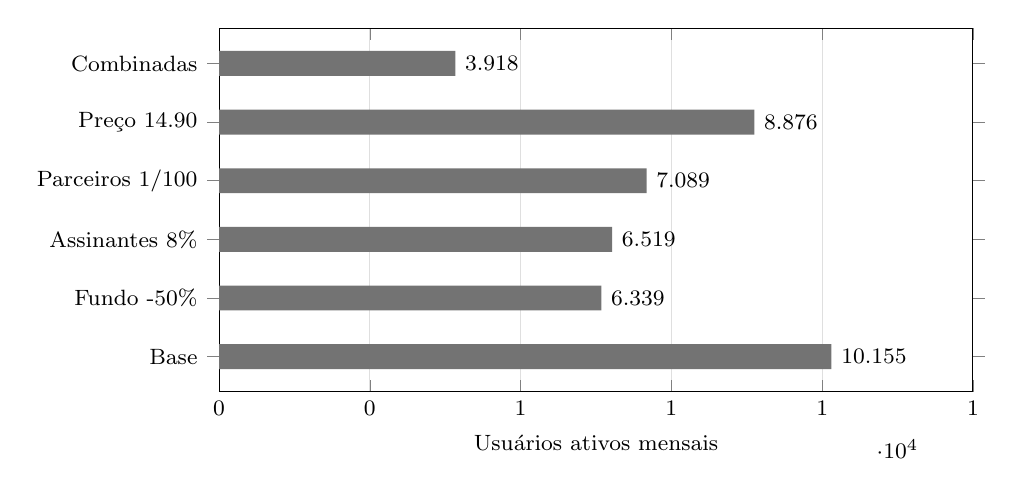
\begin{tikzpicture}
\begin{axis}[
  xbar, width=0.92\textwidth, height=6.2cm, bar width=9pt,
  xmin=0, xmax=12500, xlabel={Usuários ativos mensais},
  symbolic y coords={Combinadas,Preço 14.90,Parceiros 1/100,Assinantes 8\%,Fundo -50\%,Base},
  ytick=data, y dir=reverse,
  nodes near coords={\pgfmathprintnumber[fixed,precision=0,set thousands separator={.}]{\pgfplotspointmeta}},
  nodes near coords align={horizontal},
  every node near coord/.append style={font=\footnotesize},
  tick label style={font=\footnotesize}, label style={font=\footnotesize},
  xtick distance=2500, xmajorgrids, grid style={gray!25}, enlarge y limits=0.12,
  xticklabel={\pgfmathprintnumber[fixed,precision=0,set thousands separator={.}]{\tick}}
]
\addplot[fill=black!55, draw=none] coordinates {(3918,Combinadas) (8876,Preço 14.90) (7089,Parceiros 1/100) (6519,Assinantes 8\%) (6339,Fundo -50\%) (10155,Base)};
\end{axis}
\end{tikzpicture}
\fonteautores
\end{figure}

A leitura é direta. Nenhuma alavanca isolada leva o cenário B ao equilíbrio em escala próxima à trajetória-alvo; a combinação das três mais eficazes (fundo reduzido à metade, 8\% de assinantes e um parceiro pagante para cada cem usuários) reduz o equilíbrio de 10.155 para cerca de 3.918 usuários. Isso confirma que a escalabilidade da \projeto{} depende menos de volume bruto do que da qualidade da receita por usuário.

\begin{table}[htb]
\centering
\caption{Trajetória-alvo de usuários e resultado mensal simulado (R\$/mês)}
\label{tab:trajetoria}
\fontsizetable
\begin{tabularx}{\textwidth}{L{1.4cm} L{2.2cm} Y Y Y Y}
\toprule
\textbf{Mês} & \textbf{Usuários ativos} & \textbf{A, base, com convênio} & \textbf{A, base, sem convênio} & \textbf{B, base, com convênio} & \textbf{B, alavancas combinadas, com convênio}\\
\midrule
3 & 300 & 98,60 & -1.311,40 & -5.401,40 & -5.139,55\\
6 & 800 & 372,65 & -1.037,35 & -5.127,35 & -4.429,09\\
12 & 1.500 & 756,32 & -653,68 & -4.743,68 & -3.434,45\\
18 & 2.700 & 1.414,04 & 4,04 & -4.085,96 & -1.729,35\\
24 & 5.000 & 2.674,67 & 1.264,67 & -2.825,33 & 1.538,77\\
\bottomrule
\end{tabularx}
\fontetexto{simulação dos autores (Apêndice A); custos fixos mantidos constantes, o que é premissa otimista para trajetórias longas}
\end{table}


A trajetória-alvo da Tabela~\ref{tab:trajetoria} (300 usuários no mês 3, 800 no mês 6, 1.500 no mês 12, cerca de 2.700 no mês 18 e 5.000 no mês 24) implica crescimento mensal aproximado de 20\% entre os meses 3 e 12 e de 11\% entre os meses 12 e 24. Na simulação, o cenário enxuto sem convênio só se torna positivo por volta do mês 18, e o cenário com equipe remunerada só alcança resultado positivo no mês 24 se as alavancas combinadas forem atingidas. Como os custos fixos foram mantidos constantes, esses resultados são otimistas e devem ser lidos como limite superior.
